\documentclass[a4paper]{article}

\usepackage[english]{babel}
\usepackage[utf8x]{inputenc}
\usepackage{amsmath}
\usepackage{amsfonts}
\usepackage{graphicx}
\usepackage[colorinlistoftodos]{todonotes}

\title{CS 5785 -- Applied Machine Learning -- Lec.\ 18}
\author{Prof.\ Nathan Kallus, Cornell Tech\\Scribe: TBD}
\date{Nov.\ 2, 2017 (Under construction)}

\begin{document}
\maketitle



\section{Boosting}

\subsection{Synthetic Example (Continued)}
Picking up where we left off last lecture, if we apply Adaboost to this problem, we see in Fig.~\ref{fig:boost} we get down to around $6\%$ error after $400$ iterations.  Recall that a single stump had a test error just slightly better than chance.  Through a boosted combination of these very simple classifiers, we achieve a dramatic reduction in error rate.

\begin{figure}
\centering
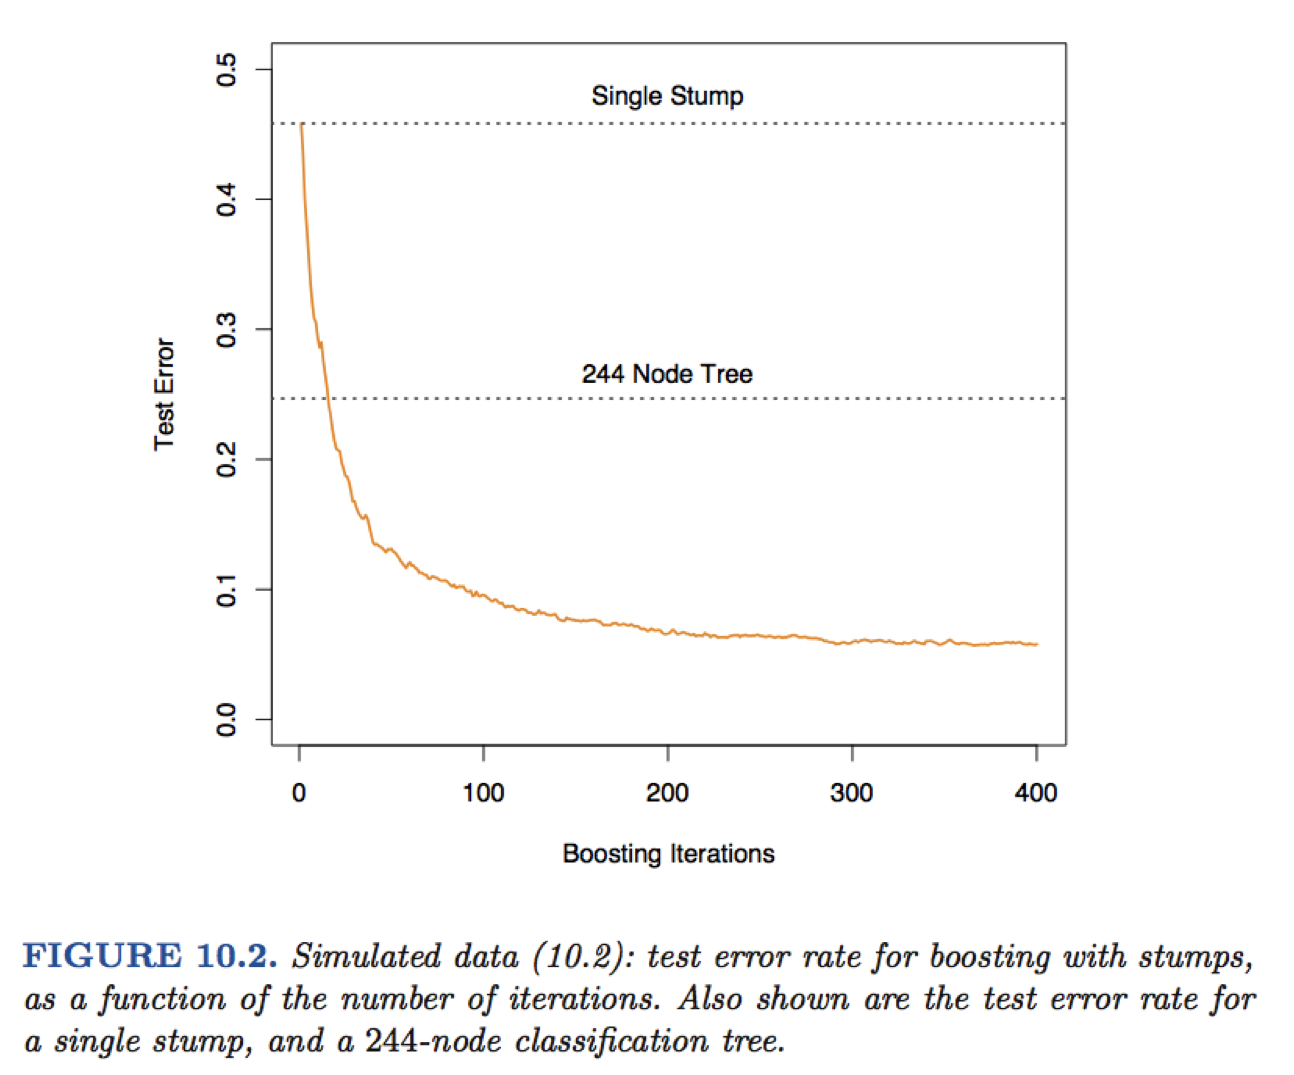
\includegraphics[width=0.8\textwidth]{fig10_2.png}
\caption{\label{fig:boost}Fig 10.2}
\end{figure}

Let's now take a closer look at how to arrive at the Adaboost algorithm.

\subsection{Loss Function}
Adaboost uses an exponential loss function:
$$
L\left( y, f(x) \right) = \exp\left( -yf(x) \right)
$$
where $f$ is the raw prediction.

We use thresholding, i.e., compute sign$(f)$, to get the class prediction from $f$. 
\begin{figure}
\centering
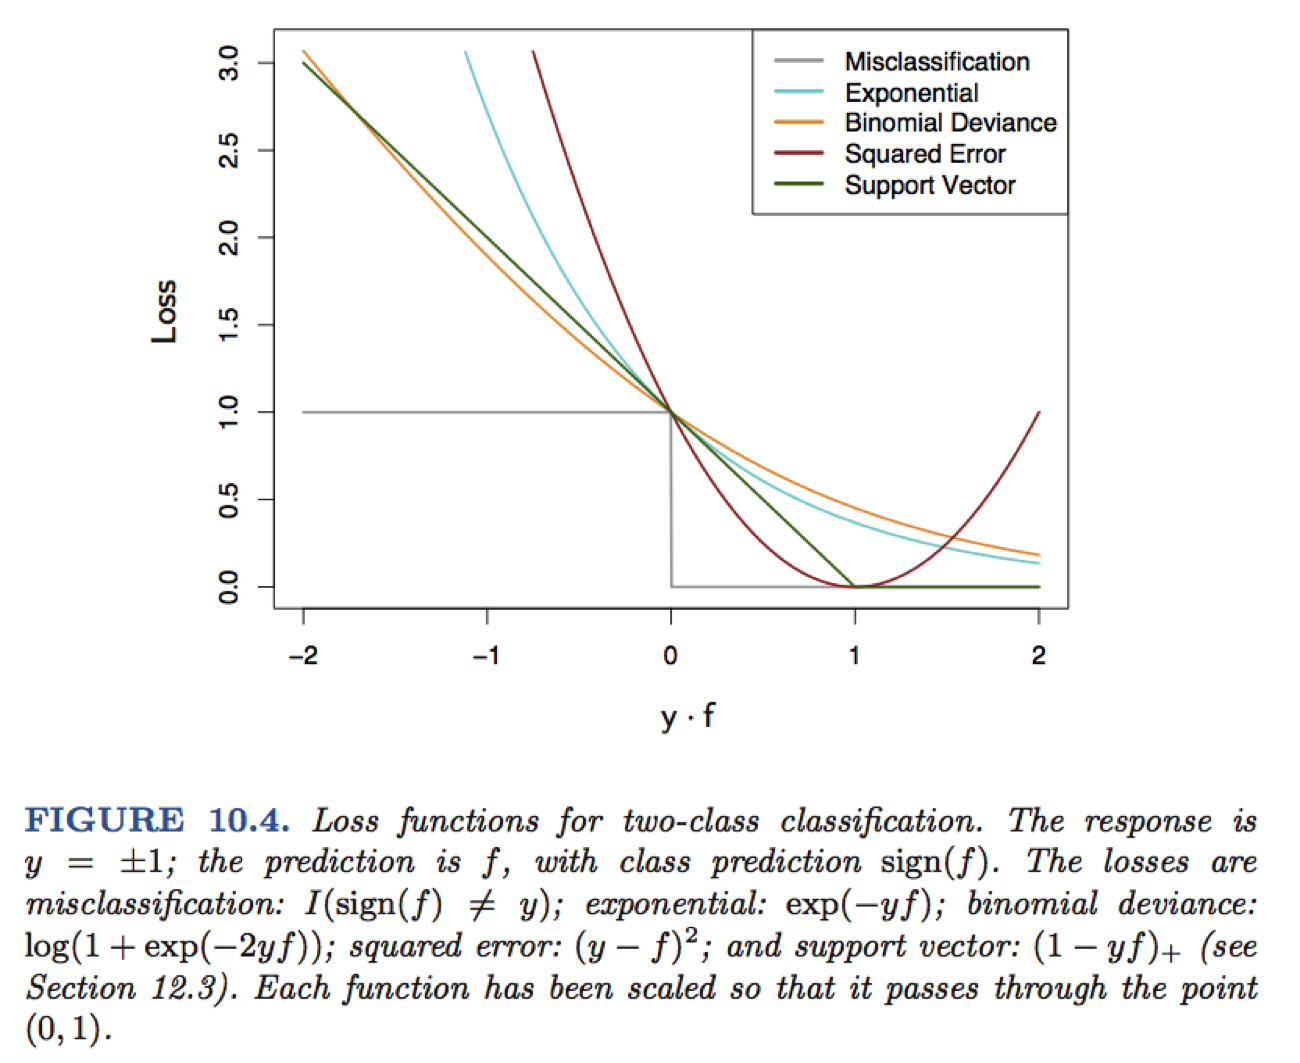
\includegraphics[width=0.8\textwidth]{fig10_4.png}
\caption{\label{fig:boost2}Fig 10.4}
\end{figure}

Fig.~\ref{fig:boost2} shows a plot of the exponential loss as a function of $y$ times $f$.
Recall that when $y=1$, we want $f$ to be positive, and when $y=-1$, we want $f$ to be negative.  Essentially, for a low loss value, we want the sign of the predicted value to match the ground truth. This implies that $yf>0$ when the prediction is correct and we expect to incur relatively little loss. Hence, the ground truth y is either +1 or -1. 

Originally, the function has a soft floating point in the training phase and in order to get the hard classification we apply the sigmoid function, which gives us +/-1. Example: Suppose a training vector is -1, then we want the predictive value to be negative.  We get the loss which is less than 1.

The raw misclassification error (plotted in gray) is simply a step function, with zero loss when the classification is correct and unit loss otherwise - it tells how much loss you incur.  The exponential is a convex upper bound (for loss) on step function. The plot shows other choices of loss functions and exponential is the one that leads to the AdaBoost algorithm.

\subsection{Solving for the classifiers and weights}
We cast our problem as one of finding the classifier $G_m$ with coefficient $\beta_m$ to be added at each step. (AdaBoost is a strictly additive approach.) Assume we have the classifier from the previous iteration of boosting and we'd like to tack on a new classifier (in our case, a decision stump) with some weight.

$$
(\beta_m, G_m) = \underset{\beta, G} {\mathrm{argmin}} \sum_{i=1}^{N} \exp[-y_i(f_{m-1}(x_i) + \beta G(x_i))]
$$

We want to find the weight and classifier to obtain some improvement in each step. We can write this as follows:

\begin{equation}
(\beta_m, G_m) = \underset{\beta, G} {\mathrm{argmin}} \sum_{i=1}^{N} w_i^{(m)} \exp(-\beta y_i G(x_i))
\end{equation}
with $w_i^{(m)} = \exp(-y_i(f_{m-1}(x_i))$. Note that $w_i^{(m)}$ depends neither on $\beta$ nor $G(x)$, so we can think of it as a per-observation weight.

At each step, it ensures an improvement by weighting the mis-classifications with a higher weight so the next iteration addresses this.  The weights change on each iteration since it depends on the previous iteration.

The solution to Equation $(1)$ can be obtained in two steps. First, for any $\beta > 0$ the solution for $G_m(x)$ is the classifer that minimizes the weighted error rate in predicting $y$.  

\begin{equation}
G_m = \underset{G} {\mathrm{argmin}} \sum_{i=1}^N w_i^{(m)} I(y_i \neq G(x_i))
\end{equation}

To see this break up Equation $(1)$ into the sum of two parts (the correctly predicted data points, contributing less to the cost, and the incorrect data points, contributing more):
$$e^{-\beta} \sum_{y_i = G(x_i)} w_i^{(m)} + e^\beta \sum_{y_i \neq G(x_i)} w_i^{(m)}$$

which we can rewrite $G_m$ as: 

$$(e^\beta-e^{-\beta}) \sum_{i=1}^N w_i^{(m)} I(y_i \neq G(x_i)) + e^{-\beta} \sum_{i=1}^N w_i^{(m)}$$

Note: on any given iteration one will get some correct and some incorrect results. When $G(x_i)$ gets a threshold, then matching is conducted - it incurs a cost; positive when you get it correctly, negative when you get it wrong. In the cases when one gets it correct one gets a sum over all the weights.

Plug this $G_m$ into Equation $(1)$ and solve for $\beta$ we get:

$$
\beta_m = \frac{1}{2} \log \frac{1-err_m}{err_m}
$$
$\beta_m$ is the weight on the weak learner that we're adding onto the new classifier (it is possible for $\beta_m$ to be zero), and the ${err_m}$ is the minimized weighted error rate:
$$
err_m = \frac{\sum_{i=1}^{N} w_i^{(m)} I(y_i \neq G(x_i))}{\sum_{i=1}^{N} w_i^{(m)}}
$$
If $err_m = 0.5$ (it's performing at chance) then the weight is $0$ so the stump doesn't get added, which is what we want.  

Before we do any iterations of boosting, the only notion of error was the sum over an indicator of any errors taking place.  Once we have this, the error depends on these weights.  We then use that to update the classifier.

We update our classifier as follows.
$$f_m(x) = f_{m-1}(x) + \beta_m G_m(x) $$
with weights for the next iteration defined as
$$w_i^{(m+1)} = w_i^{(m)} e^{-\beta_m y_i G_m(x_i)}$$

We use the fact that 

$$-y_i G_m(x_i) = 2 \cdot I(y_i \neq G_m(x_i)) - 1$$
where it becomes 1 if an error occurs and 0 if its correct. Then we get
$$w_i^{(m+1)} = w_i^{(m)} \cdot e^{\alpha_m I(y_i \neq G_m(x_i))} e^{-\beta_m}$$
where $\alpha_m = 2 \beta_m$ is the quantity in line $2c$ of the Adaboost algorithm, which is shown in Figure 3 from Lecture 17.

We can drop the factor $e^{\beta_m}$ since it won't affect our maximization problem so we get line 2d shown in Figure 3 from Lecture 17: 
$$
\text{set} \: w_i \leftarrow w_i \: \exp[\alpha_m I(y_i \neq G_m(x_i))], \: i = 1, 2, ..., N
$$

You take your weights from the last iteration, which emphasize the misclassified ones, and then try your best to solve for the parameters for the next stump.  Initially, you have many weak classifiers, but at the end of AdaBoost you produce a strong classifier that's the weighted combination of these weak classifiers.  In Fig.\ ~\ref{fig:boost3}, you can see how performance improves for our motivating example.

\begin{figure}
\centering
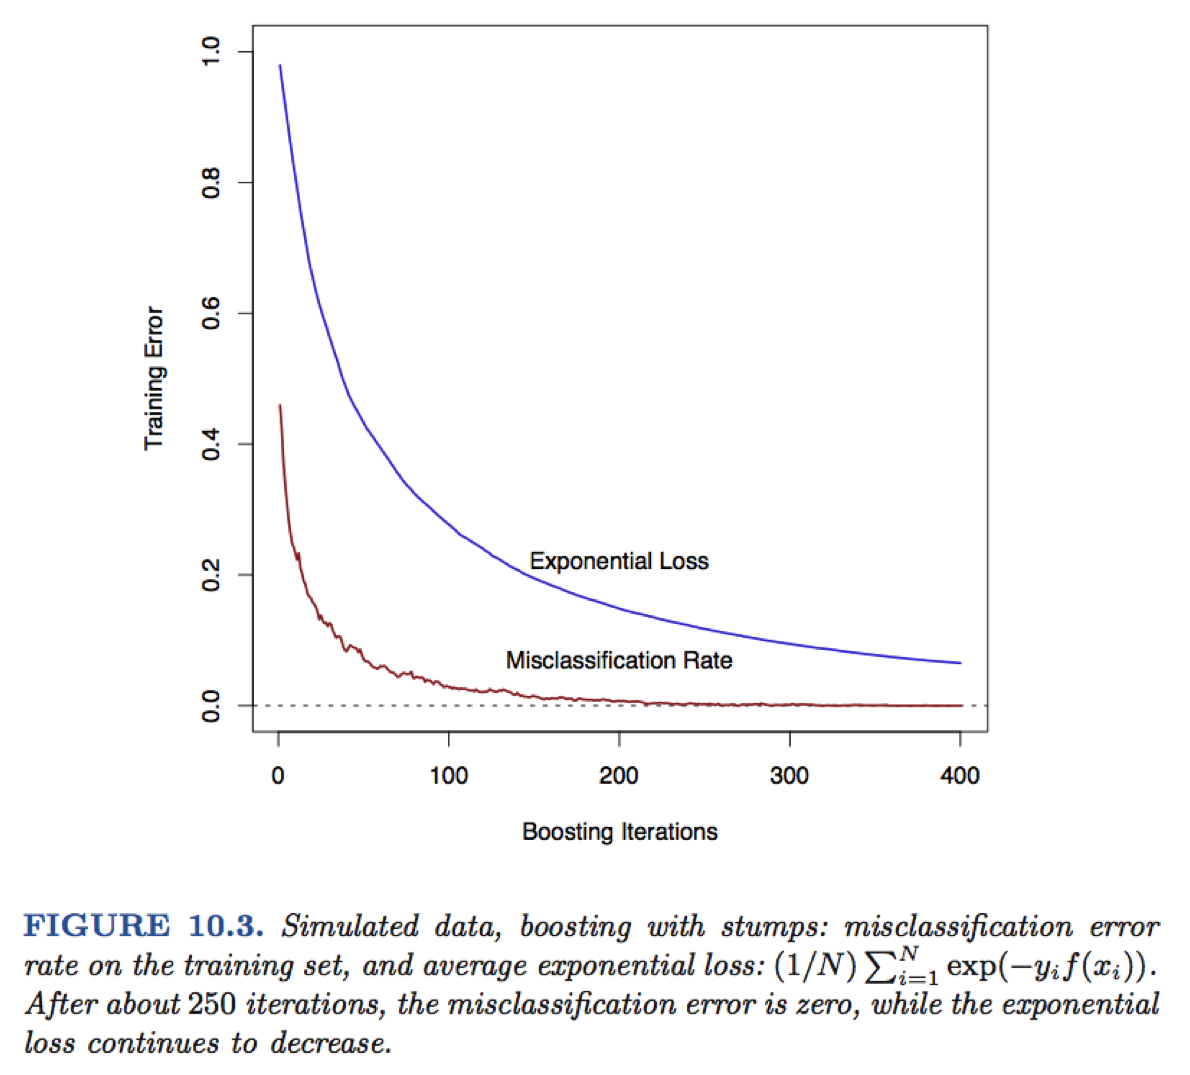
\includegraphics[width=1.0\textwidth]{fig10_3.png}
\caption{\label{fig:boost3}Fig 10.3}
\end{figure}

Fig.\ ~\ref{fig:anim}, takes us through some of the iterations of AdaBoost, step by step.  For a stump, you pick a variable (choice of 2 here) and threshold by sweeping. Now you have weights for each observation, bigger ones for the ones misclassified, so you do this again.  The final strong classifier is a weighted combination of all these regions.

\begin{figure}
\begin{tabular}{cc}
  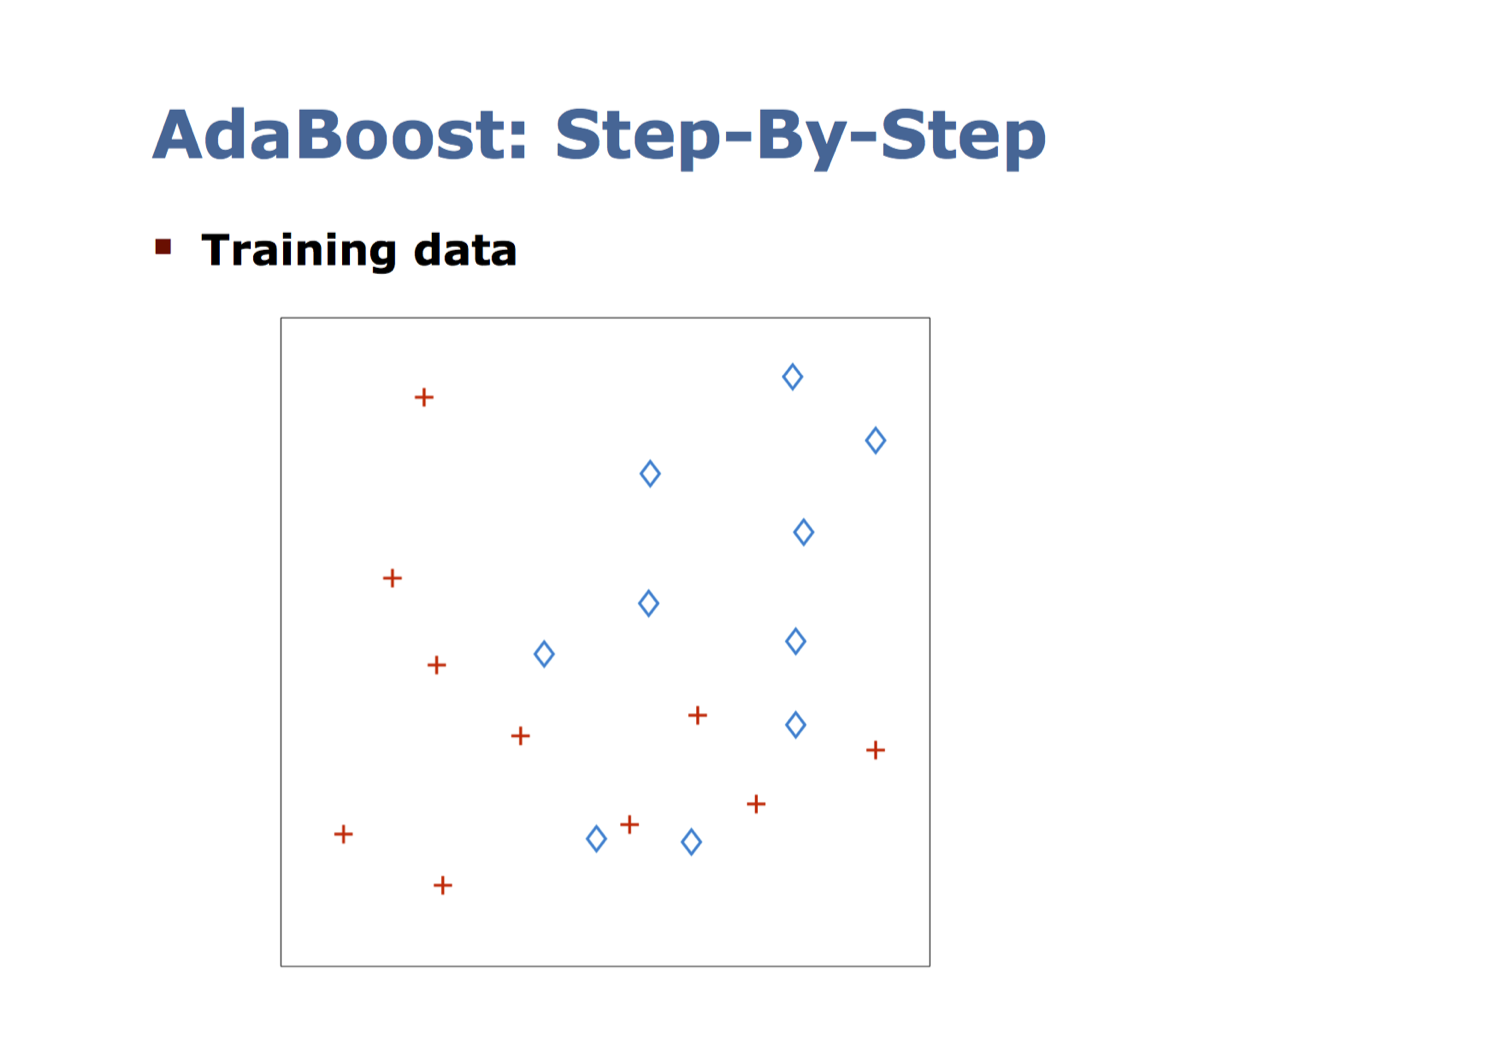
\includegraphics[width=65mm]{adaboost1.png} &   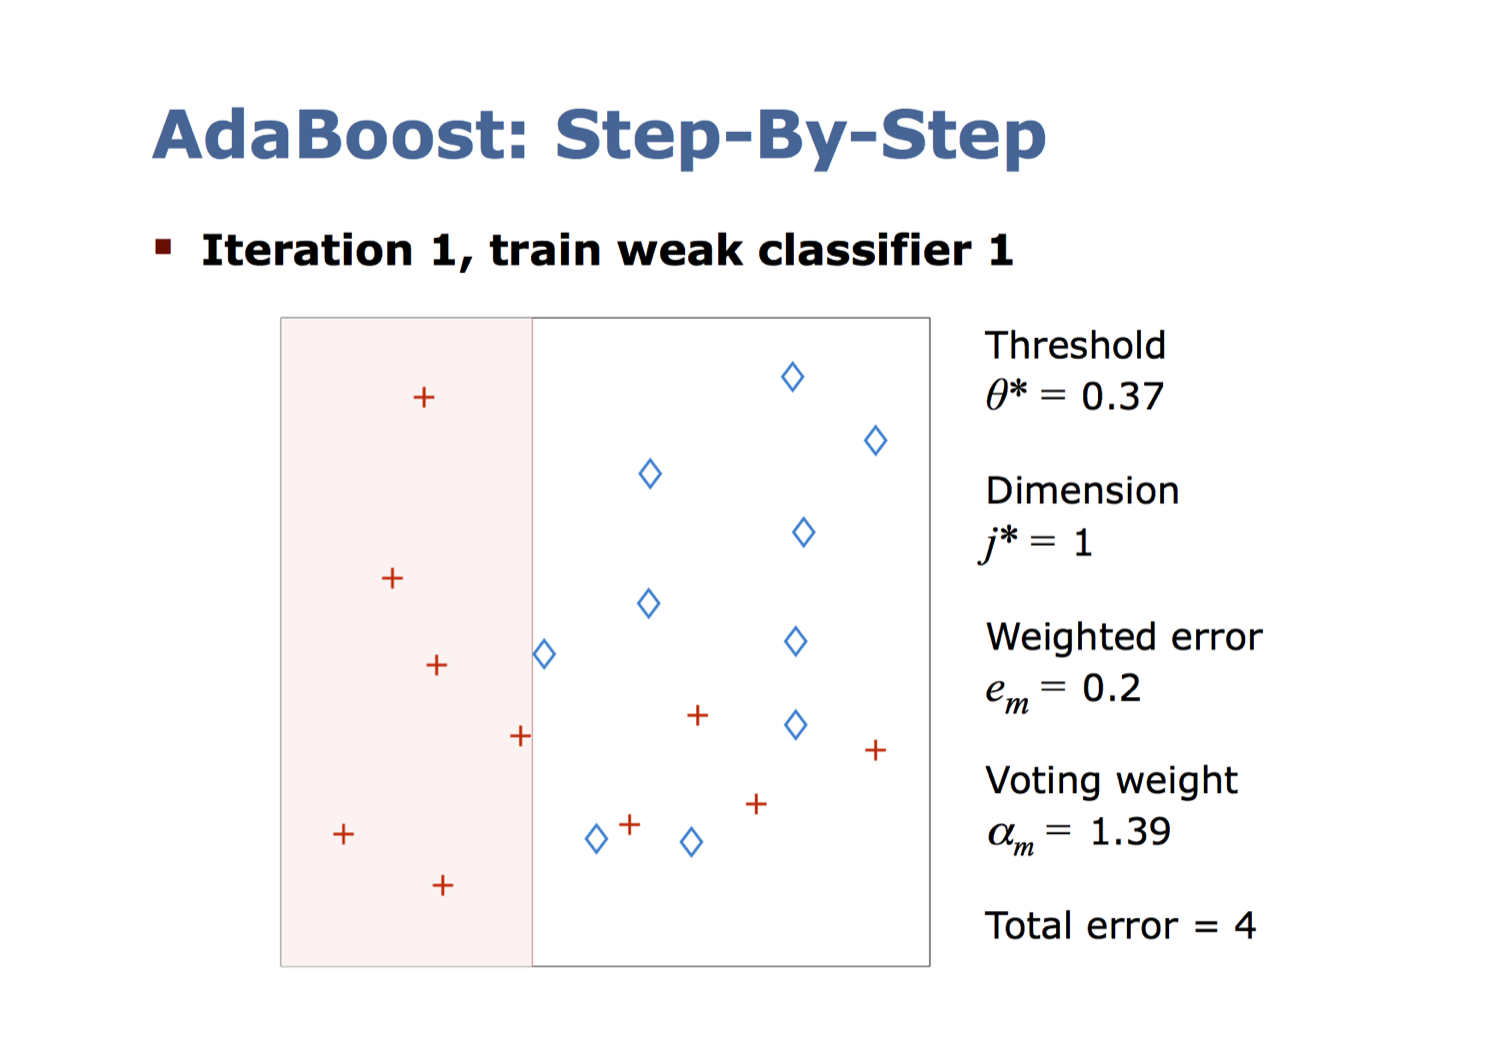
\includegraphics[width=65mm]{adaboost2.png} \\
(a) first & (b) second \\[6pt]
 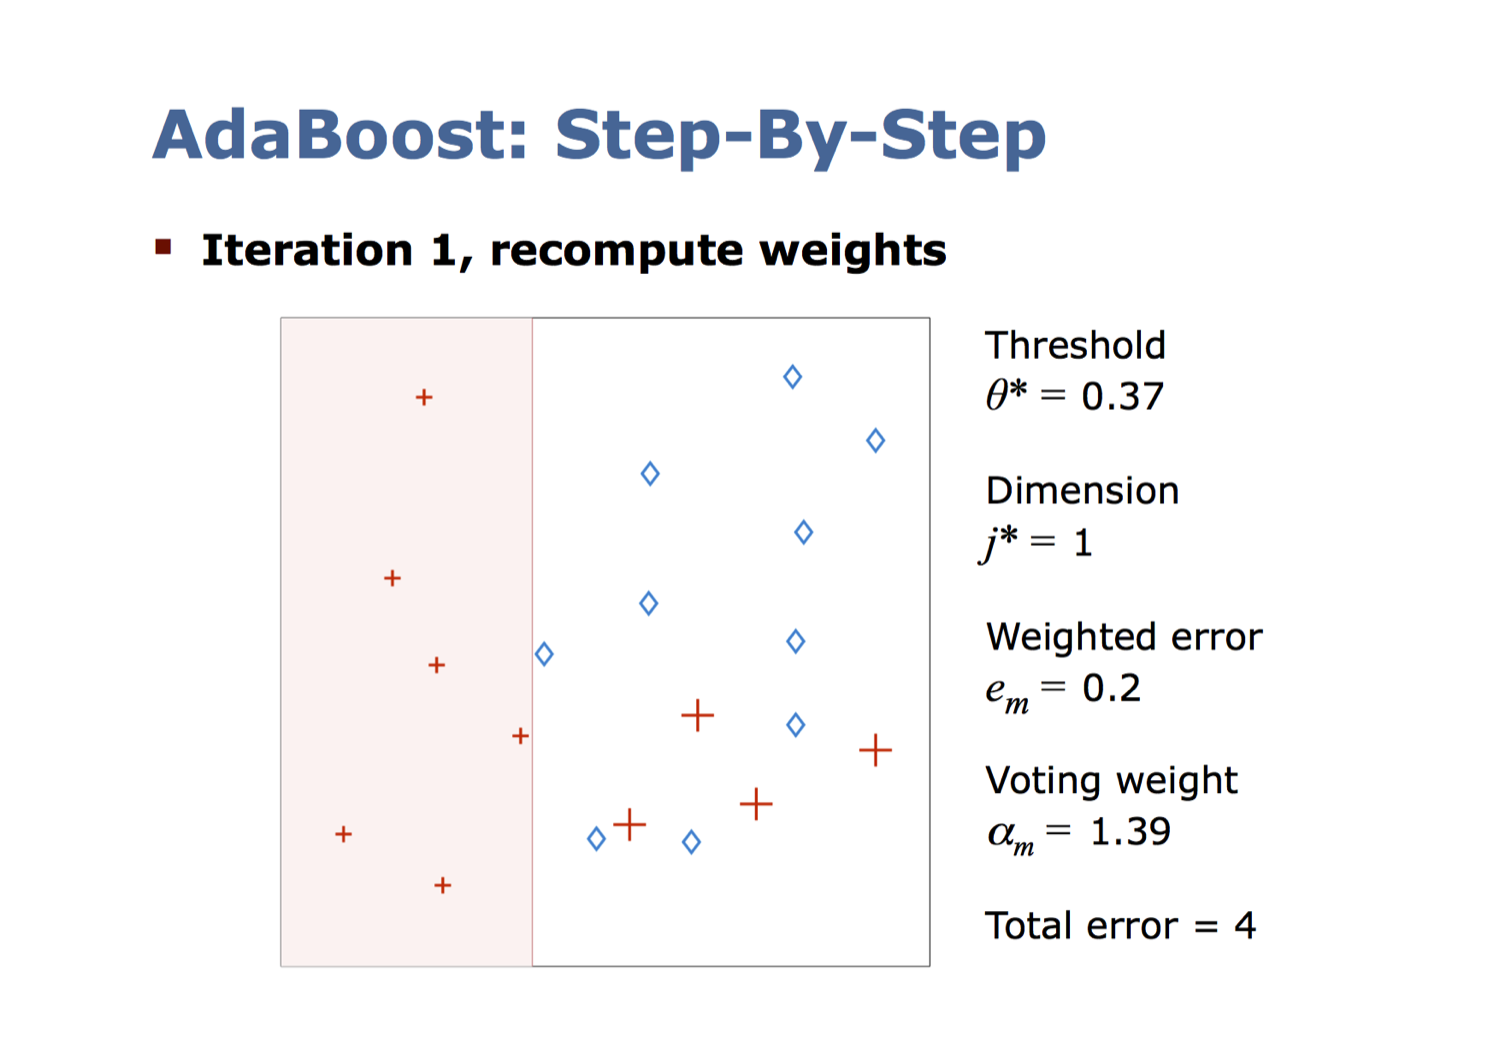
\includegraphics[width=65mm]{adaboost3.png} &   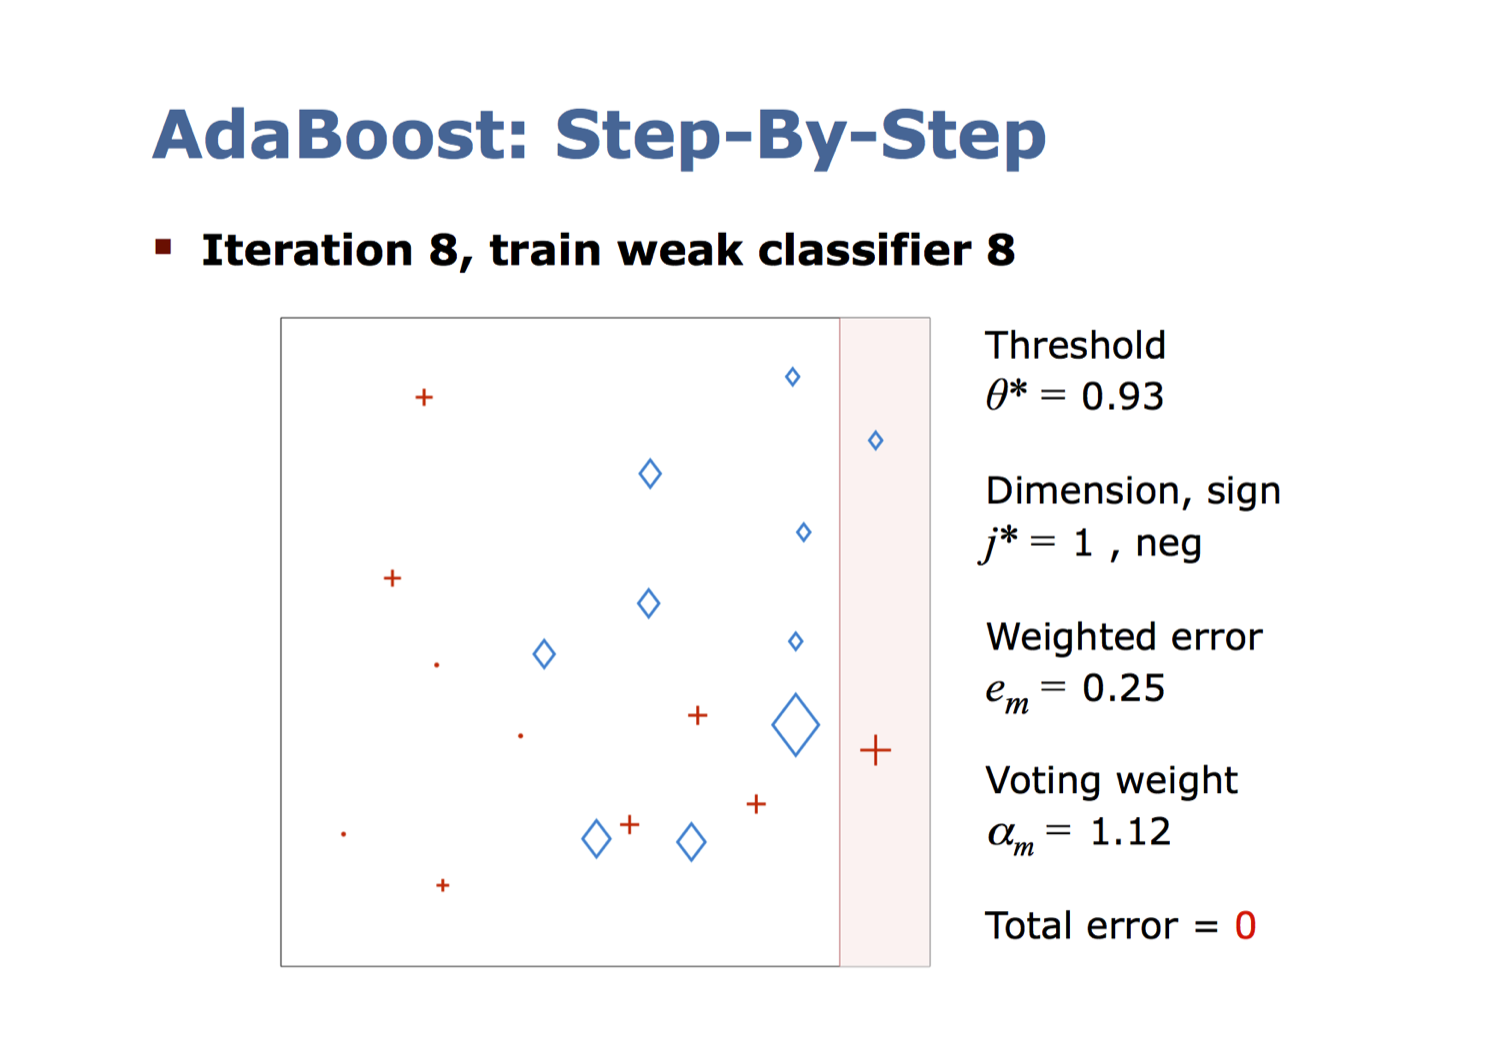
\includegraphics[width=65mm]{adaboost4.png} \\
(c) third & (d) fourth \\[6pt]
 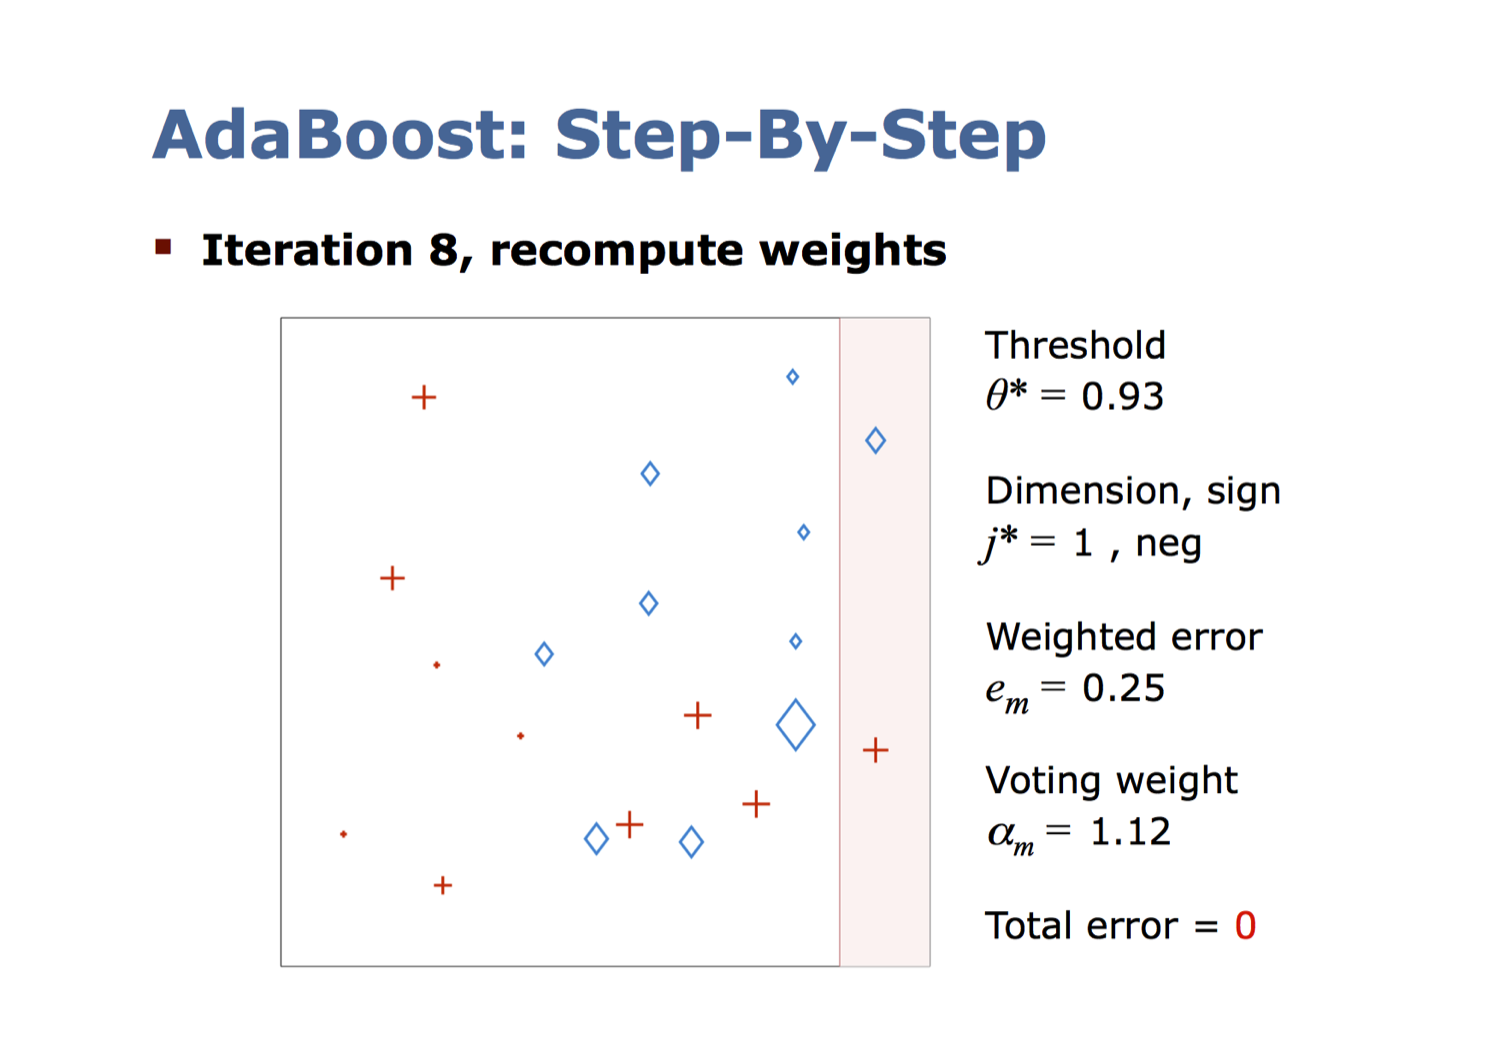
\includegraphics[width=65mm]{adaboost5.png} &
  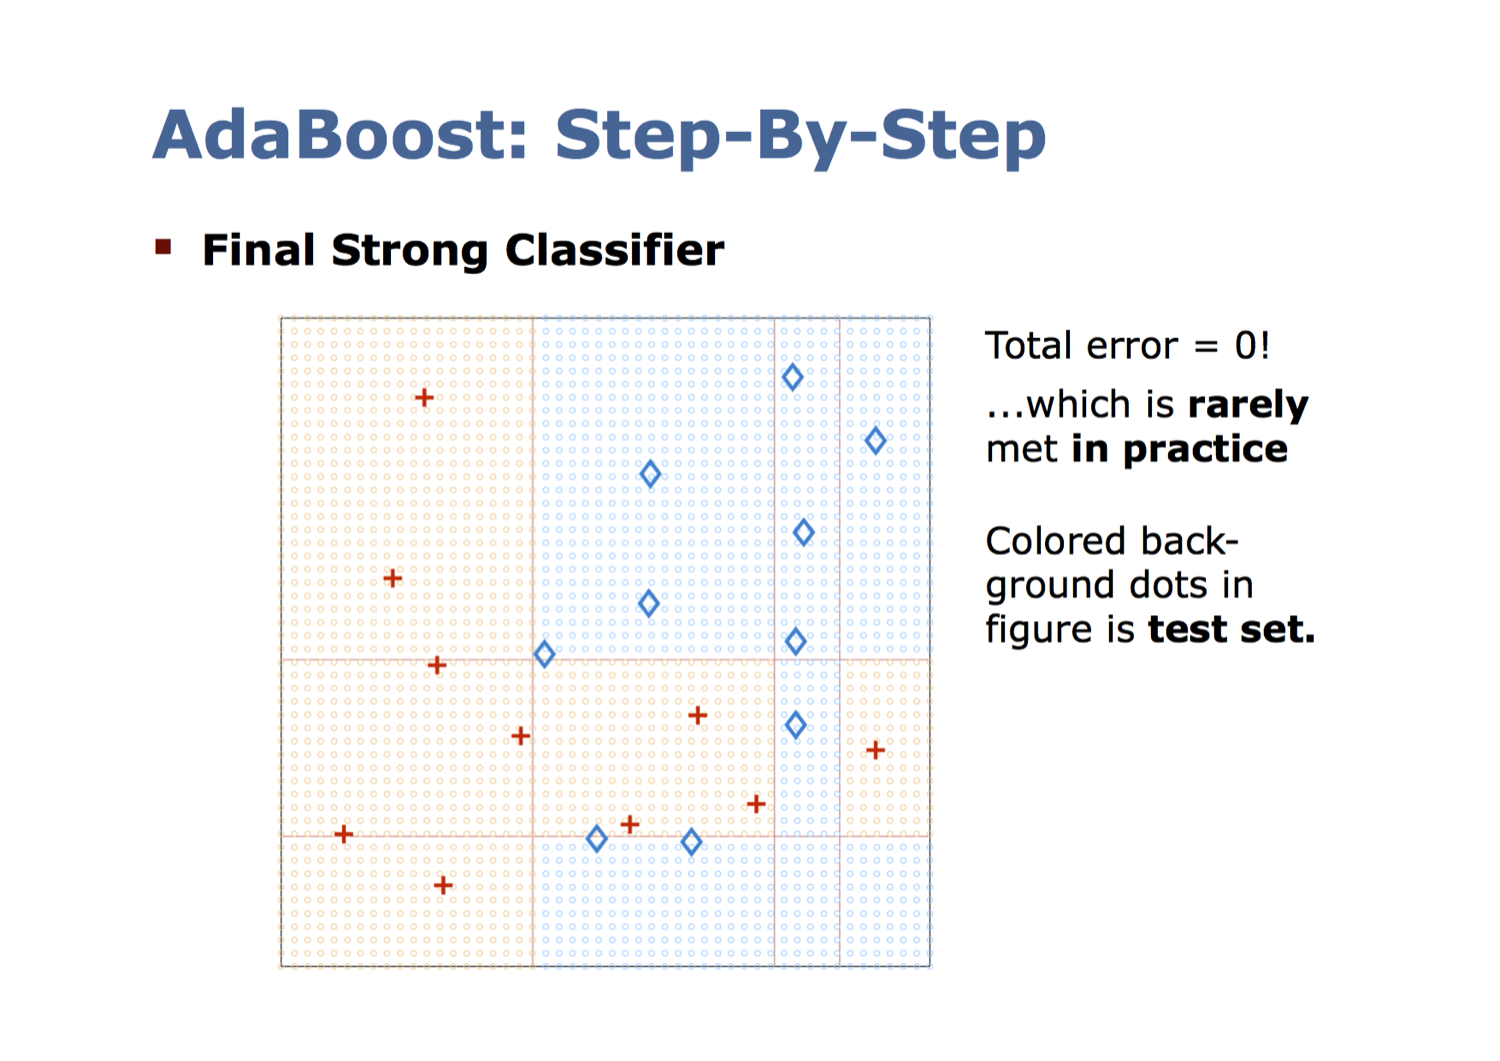
\includegraphics[width=65mm]{adaboost6.png} \\
(e) fifth & (f) sixth \\[6pt]
\multicolumn{2}{c}{}
\end{tabular}
\caption{\label{fig:anim}Animation of Adaboost}
\end{figure}

Fig.\ ~\ref{fig:boost4}, you see the same thing basically with the result of a final strong classifier.  You get a weighted combination and just threshold half-way.

\begin{figure}
\centering
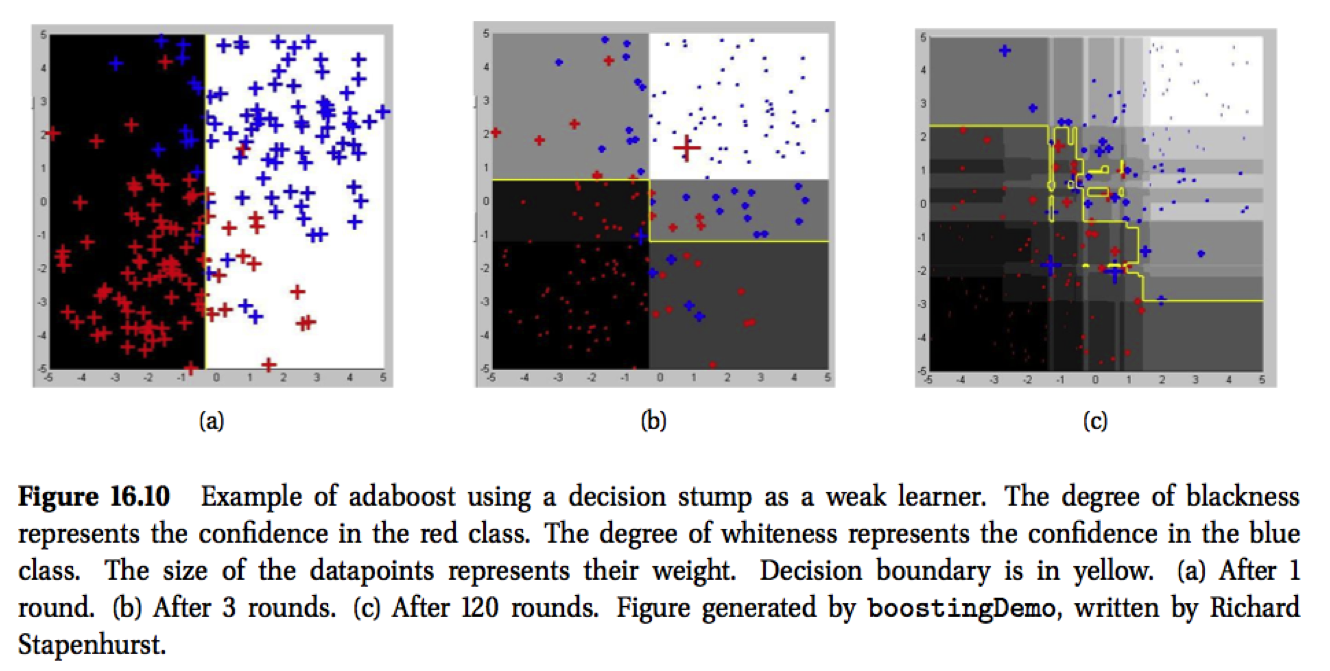
\includegraphics[width=1.0\textwidth]{fig16_10.png}
\caption{\label{fig:boost4}Fig 16.10}
\end{figure}

\section{Viola-Jones}

Recall that boosting is a meta-algorithm that sits on top of a weak classifier. For face detection, as seen Fig. ~\ref{fig:boost5}, advocated the use of a stump defined with a Haar-like wavelet.

\begin{figure}
\centering
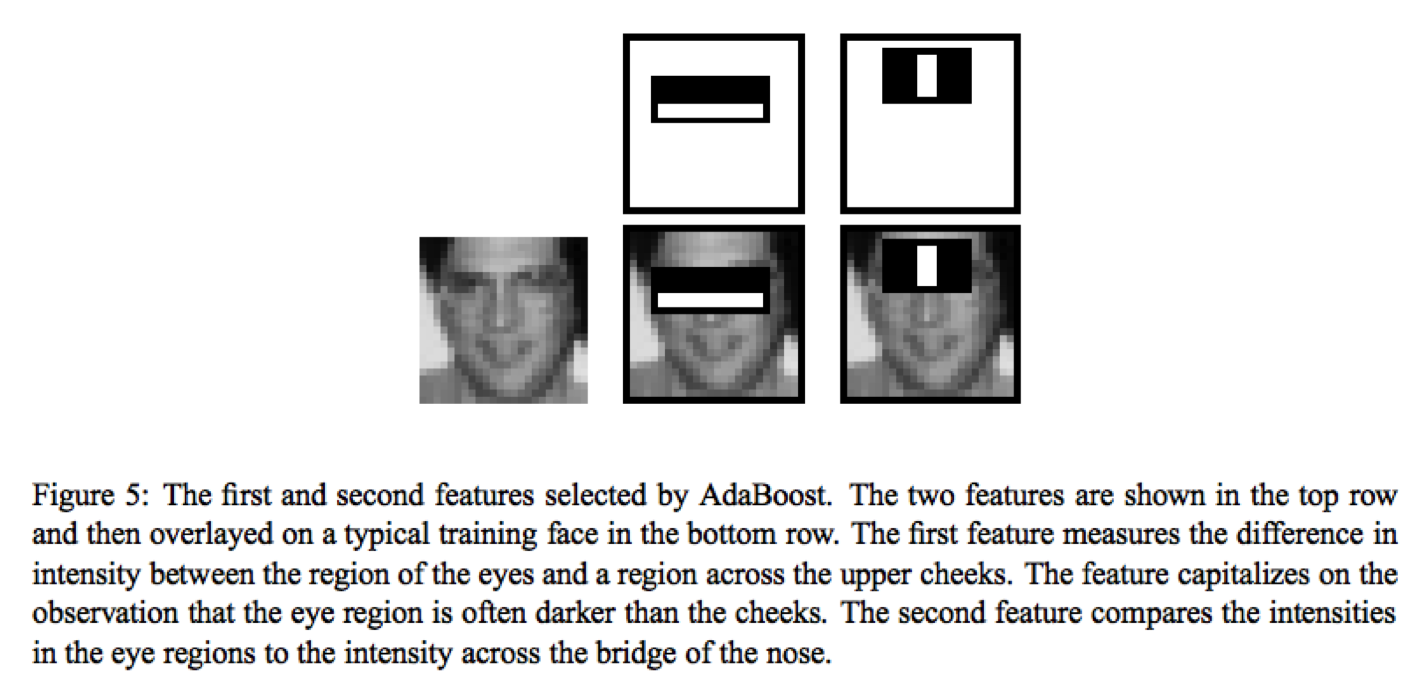
\includegraphics[width=1.0\textwidth]{fig5.png}
\caption{\label{fig:boost5}Fig 5}
\end{figure}

A Haar-like wavelet involves picking an overall box size for the size of a face, say $96 \times 96$ with a fixed scale, that you then slide around the image ("cascaded implementation").  The Haar-like wavelet are a set of boxes that are $+1, -1$ and everywhere else is $0$.  These are the features that operationalize the stump, which is created using the inner product with the Haar-like wavelet and a cropped section of the image.  

When you encounter an image of a face, a Haar-like wavelet finds a product between all the pixel values inside the window. It will compute the distance. 

\begin{figure}
\centering
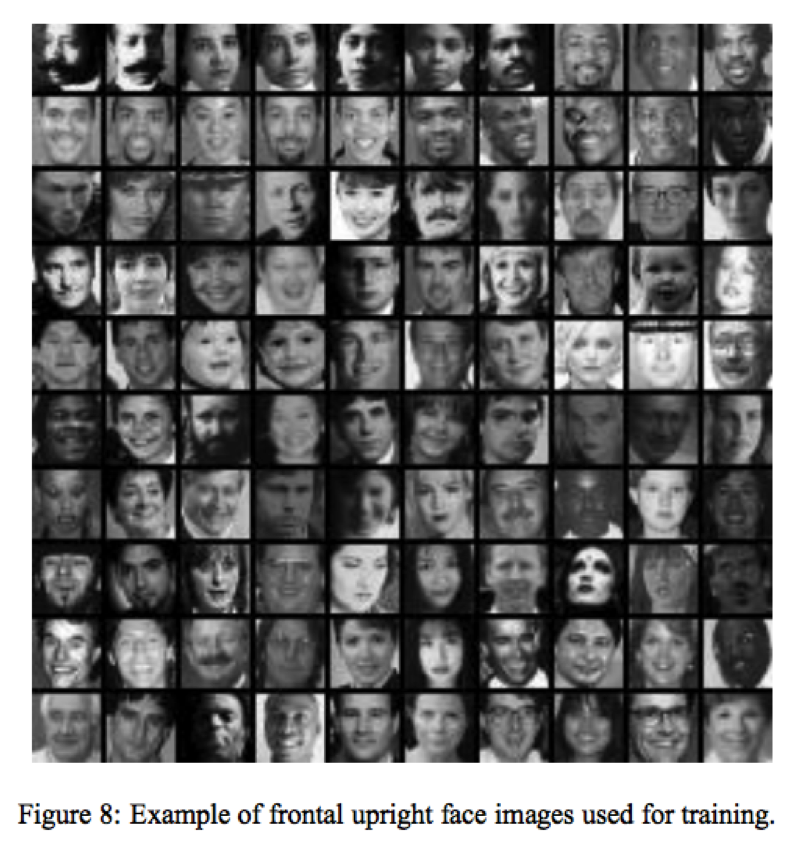
\includegraphics[width=1.0\textwidth]{fig8.png}
\caption{\label{fig:boost6}Training Images}
\end{figure}

\begin{figure}
\centering
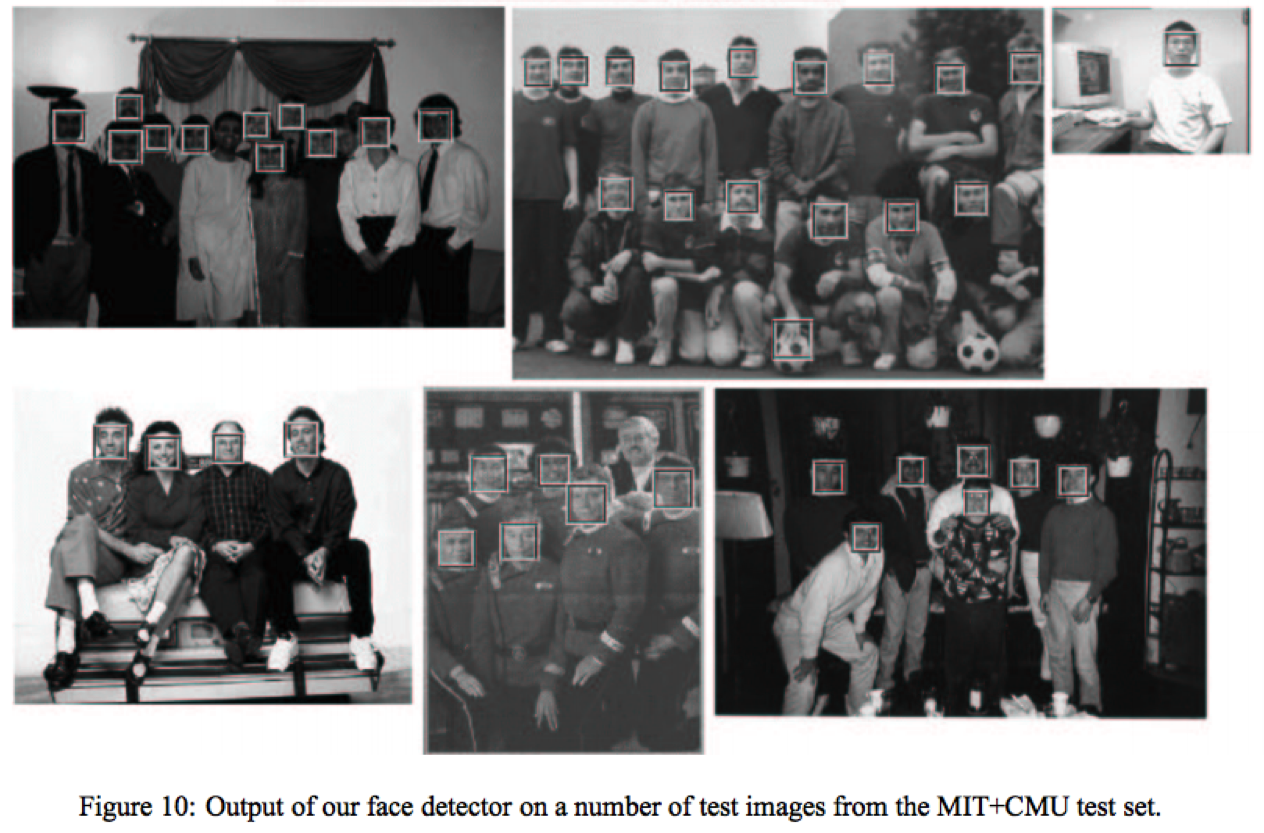
\includegraphics[width=1.0\textwidth]{fig10.png}
\caption{\label{fig:boost7}Test Images}
\end{figure}

\begin{figure}
\centering
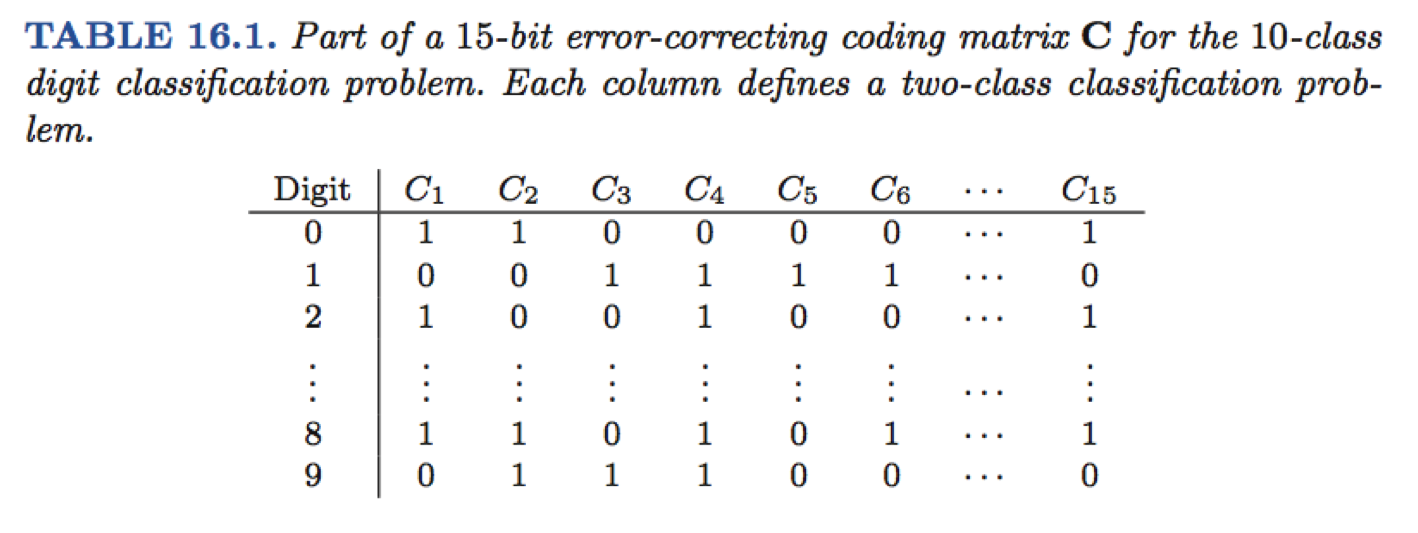
\includegraphics[width=1.0\textwidth]{table16_1.png}
\caption{\label{fig:boost8}Table 16.1}
\end{figure}

Viola-Jones method is super fast. Especially when compared to Neural Networks for the face bounding problem in 1999, around when Viola-Jones was introduced. Fig.\ ~\ref{fig:boost6} shows the training set of images and Fig.\ ~\ref{fig:boost7} shows the performance on different test images. Some of the things they used to make this efficient were:

\begin{enumerate}
\item Cascade: early rejection - created multilevel cascade with many boosted classifiers.
\item Integral image trick: summed area table that is precomputed so the value is the sum of all pixel values inside a rectangle.
\item Multiscale search: also key to that faces can be huge selfies.
\end{enumerate}

Boosting is still king in face detection.  Random forests does well with multi-class classification.

Ada boost is a strictly additive classification method. When we are done boosting - then we threshold it at zero. Ada boost doesn’t overfit. In most methods one needs to be careful how long one trains the model. For most methods when the training error is close to zero - the validation error can easily go up. This does not happen in boosting. Boosting is so pupular since it doesn’t overfit. Increasing the iterations does no harm.

Fig.\ ~\ref{fig:boost8} shows an early example of a learning ensemble using boosting technology. Boosting can't handle multi-class.  A clever response was ECOC (error correcting output code).  We assign each digit a codeword and train the classifier to produce $0$ or $1$ for each digit.  Boosting produces bits in a code word.  Note that the rows have more bits than is neccessary and the idea is that the redundant "error-correcting" bits allow for some inaccuracies and can improve performance. In our case, for $10$ digits, you have a length $15$ code word. Then you calculate the Hamming distance to the closest codeword. This means some of the bits will get classified incorrectly but the error-correcting codes will tolerate this the best it can since the $8$ classes code words are designed to be as far apart as possible. Actually this turns out not any better than randomly assigned code words but will not be covered and left as an advanced topic.
Neural networks on the other hand requires complex arrays.

Finally, in order to use the above approaches - you needed lots of training data. 

\end{document}
